%%
%% Class homework & solution template for latex
%% Alex Ihler
%%
\documentclass[twoside,11pt]{article}
\usepackage{amsmath,amsfonts,amssymb,amsthm}
\usepackage{graphicx,color}
\usepackage{verbatim,url}
\usepackage{listings}
\usepackage{upquote}
\usepackage[T1]{fontenc}
%\usepackage{lmodern}
\usepackage[scaled]{beramono}
%\usepackage{textcomp}

% Directories for other source files and images
\newcommand{\bibtexdir}{../bib}
\newcommand{\figdir}{fig}

\newcommand{\E}{\mathrm{E}}
\newcommand{\Var}{\mathrm{Var}}
\newcommand{\N}{\mathcal{N}}
\newcommand{\matlab}{{\sc Matlab}\ }

\setlength{\textheight}{9in} \setlength{\textwidth}{6.5in}
\setlength{\oddsidemargin}{-.25in}  % Centers text.
\setlength{\evensidemargin}{-.25in} %
\setlength{\topmargin}{0in} %
\setlength{\headheight}{0in} %
\setlength{\headsep}{0in} %

\renewcommand{\labelenumi}{(\alph{enumi})}
\renewcommand{\labelenumii}{(\arabic{enumii})}

\theoremstyle{definition}
\newtheorem{MatEx}{M{\scriptsize{ATLAB}} Usage Example}

\definecolor{comments}{rgb}{0,.5,0}
\definecolor{backgnd}{rgb}{.95,.95,.95}
\definecolor{string}{rgb}{.2,.2,.2}
\lstset{language=Matlab}
\lstset{basicstyle=\small\ttfamily,
        mathescape=true,
        emptylines=1, showlines=true,
        backgroundcolor=\color{backgnd},
        commentstyle=\color{comments}\ttfamily, %\rmfamily,
        stringstyle=\color{string}\ttfamily,
        keywordstyle=\ttfamily, %\normalfont,
        showstringspaces=false}
\newcommand{\matp}{\mathbf{\gg}}




\begin{document}

\centerline{\Large Homework 2}
\centerline{Zachary DeStefano, 15247592}
\centerline{CS 273A: Winter 2015}
\centerline{\bf Due: January 20, 2015}

\section*{Problem 1}

\subsection*{Part a}

Here is the code to complete part a
\lstinputlisting[firstline=2, lastline=8]{prob1.m}

\subsection*{Part b}

Here is the code to complete part b. It does rely on the code from part a:
\lstinputlisting[firstline=9, lastline=24]{prob1.m}

\newpage

Here is the plot for part b:
\begin{figure}[h]
\centering
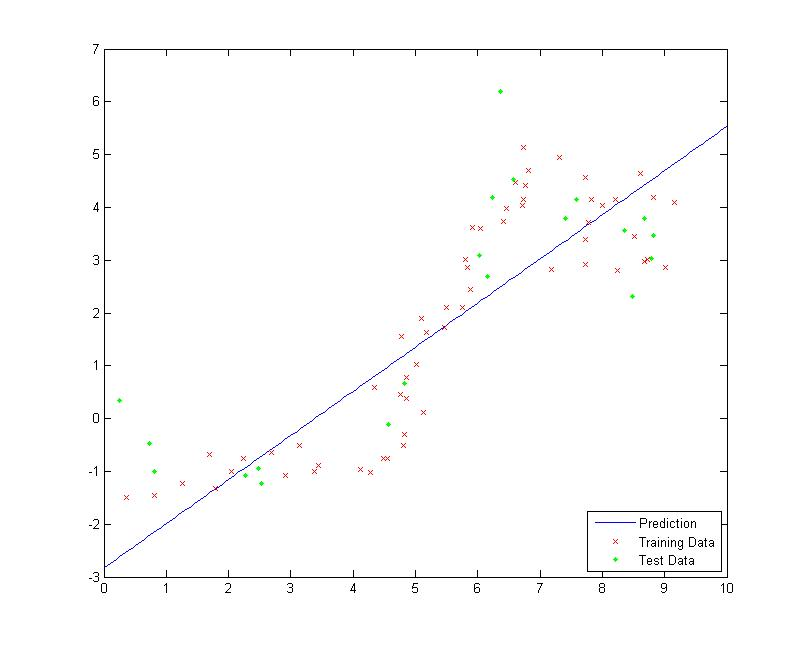
\includegraphics[width=5 in]{prob1bPlot.jpg}
\caption{The training data, test data, and the predicted values}
\end{figure}

\newpage

\subsection*{Part c}

%	For direct matlab code
%\begin{lstlisting}
%\end{lstlisting}

Here is the plot of the $f(x)$ functions and the training and test data
\begin{figure}[h]
\centering
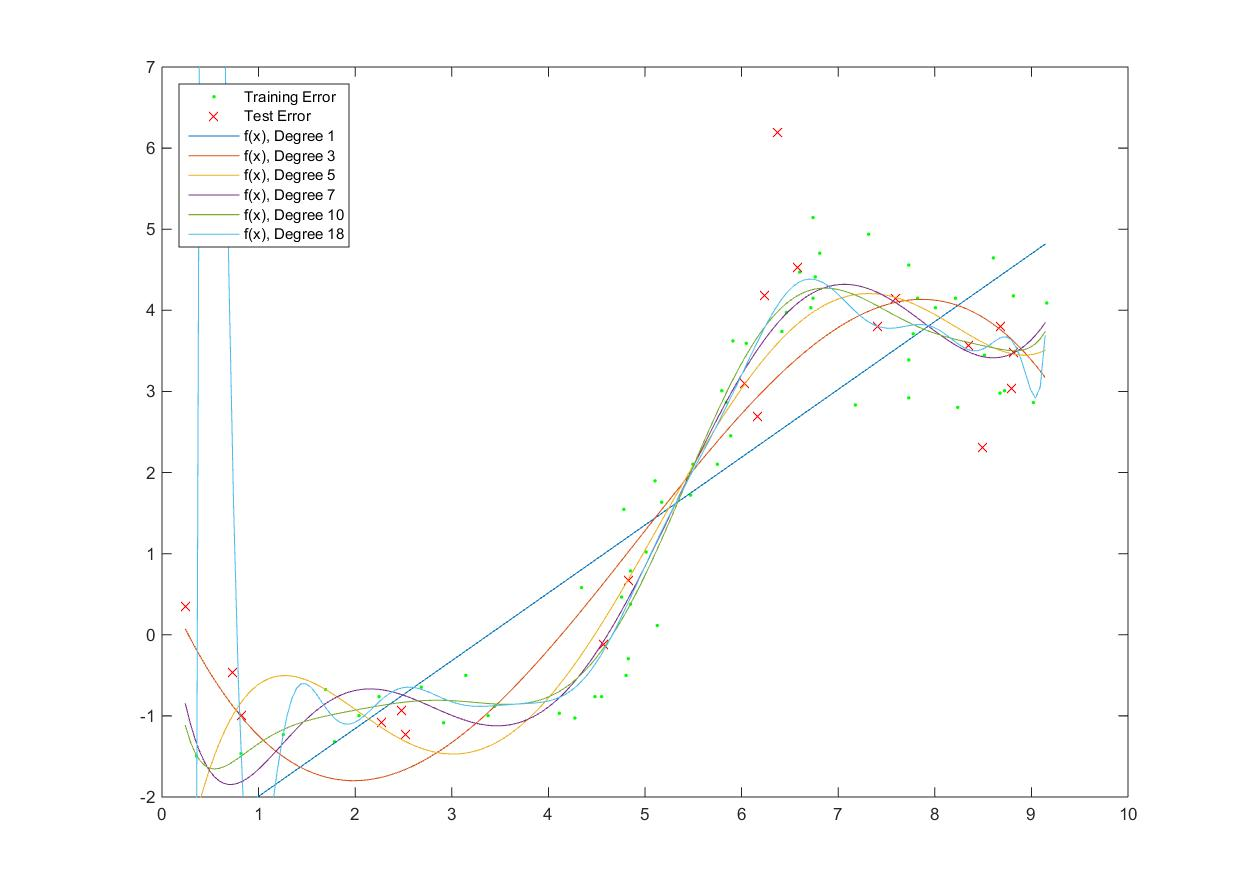
\includegraphics[width=5 in]{prob1cPlotA.jpg}
\caption{The training data, test data, and the best-fit polynomial}
\end{figure}

\newpage

Here is the plot of the training and test error
\begin{figure}[h]
\centering
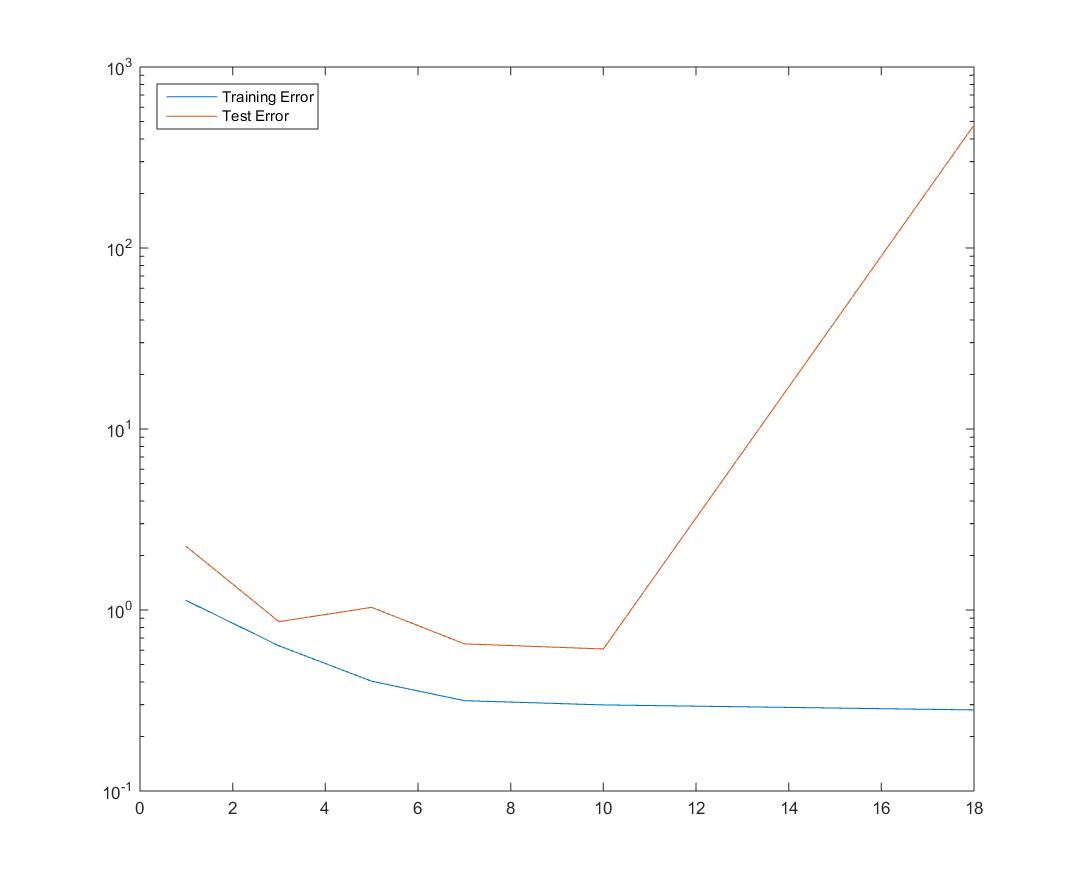
\includegraphics[width=5 in]{prob1cPlotB.jpg}
\caption{The training and test error}
\end{figure}

\newpage

This is the code used to accomplish these plots. It is a continuation of the code from part a as it uses the arrays created there. 
\lstinputlisting[firstline=30, lastline=80]{prob1.m}

\newpage

\section*{Problem 3}

This is the plot. As can be observed, the minimum average MSE occurs where $degree=7$. \\
\begin{figure}[h]
\centering
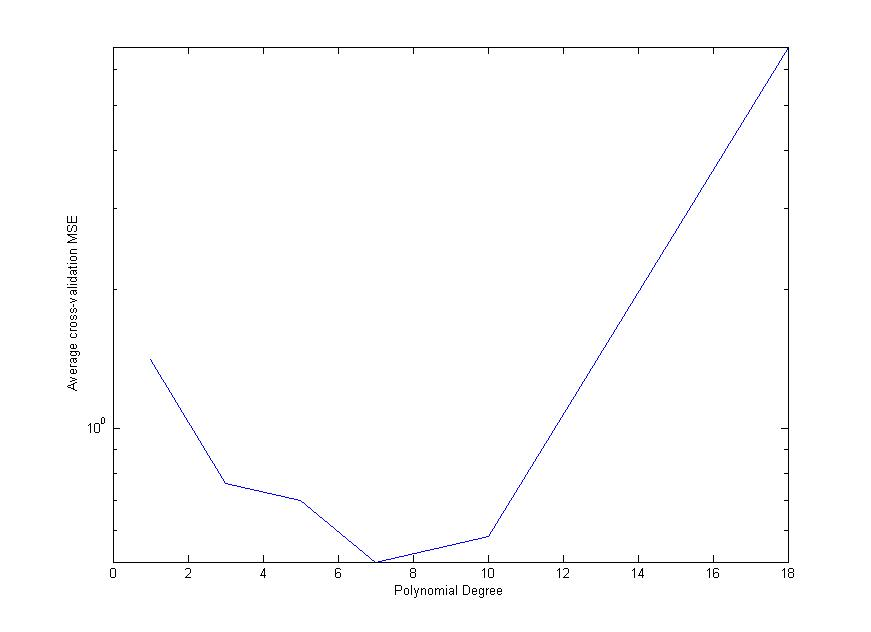
\includegraphics[width=5 in]{prob2Plot.jpg}
\caption{The average cross-validation MSE as function of polynomial degree}
\end{figure}
The average cross-validation MSE for the degree 7 polynomial was $0.5138$.\\
The test error for the degree 7 polynomial in problem 2 was $0.6502$.\\
Therefore using cross-validation reduced the test error slightly.\\
\\
Using cross-validation also changed which polynomial degree had the least test error. \\
In problem 2, the degree 10 polynomial had the least test error whereas in problem 3, \\
the degree 7 polynomial performed the best. \\
\\
\newpage
Here is the code that I used to get the numbers and the plot for problem 3
\lstinputlisting[firstline=1, lastline=43]{prob2.m}


\end{document}
